\documentclass[12pt]{article}
\usepackage[table]{xcolor}
\usepackage[margin=1in]{geometry} 
\usepackage{amsmath,amsthm,amssymb}
\usepackage[english]{babel}
\usepackage{tcolorbox}
\usepackage{enumitem}
\usepackage{hyperref}
\usepackage{listings}
\usepackage{blkarray}
\usepackage{float}
\usepackage{bm}
\usepackage{subfigure}
\usepackage{booktabs}
\usepackage{siunitx}
\usepackage{commath}

\setcounter{secnumdepth}{5}
\setcounter{tocdepth}{5}

\newtheorem{theorem}{Theorem}[section]
\newtheorem{corollary}{Corollary}[theorem]
\newtheorem{lemma}[theorem]{Lemma}
\newtheorem{proposition}[theorem]{proposition}
\newtheorem{exmp}{Example}[section]\newtheorem{definition}{Definition}[section]
\newtheorem{remark}{Remark}
\newtheorem{ex}{Exercise}
\theoremstyle{definition}
\theoremstyle{remark}
\bibliographystyle{elsarticle-num}

\DeclareMathOperator{\sinc}{sinc}
\DeclareMathOperator{\sign}{sign}
\newcommand{\RNum}[1]{\uppercase\expandafter{\romannumeral #1\relax}}
\newcommand{\N}{\mathbb{N}}
\newcommand{\Z}{\mathbb{Z}}
\newcommand{\R}{\mathbb{R}}
\newcommand{\E}{\mathbb{E}}
\newcommand{\matindex}[1]{\mbox{\scriptsize#1}}
\newcommand{\V}{\mathbb{V}}
\newcommand{\Q}{\mathbb{Q}}
\newcommand{\K}{\mathbb{K}}
\newcommand{\C}{\mathbb{C}}
\newcommand{\prob}{\mathbb{P}}

\lstset{numbers=left, numberstyle=\tiny, stepnumber=1, numbersep=5pt}

%\pagenumbering{gobble}
%\setcounter{secnumdepth}{0} % This line removes the numbers in the titles.

\begin{document}
\title{Self-repairing 3D printer: Ideas}
\author{Renzo Miguel Caballero Rosas\\
\url{Renzo.CaballeroRosas@kaust.edu.sa}\\
\url{CaballeroRenzo@hotmail.com}\\
\url{CaballeroRen@gmail.com}} 
%\date{\vspace{-5ex}}
\maketitle

\tableofcontents

\section{Idea 1: Correcting using Encoder}

\begin{figure}[ht!]
\centering
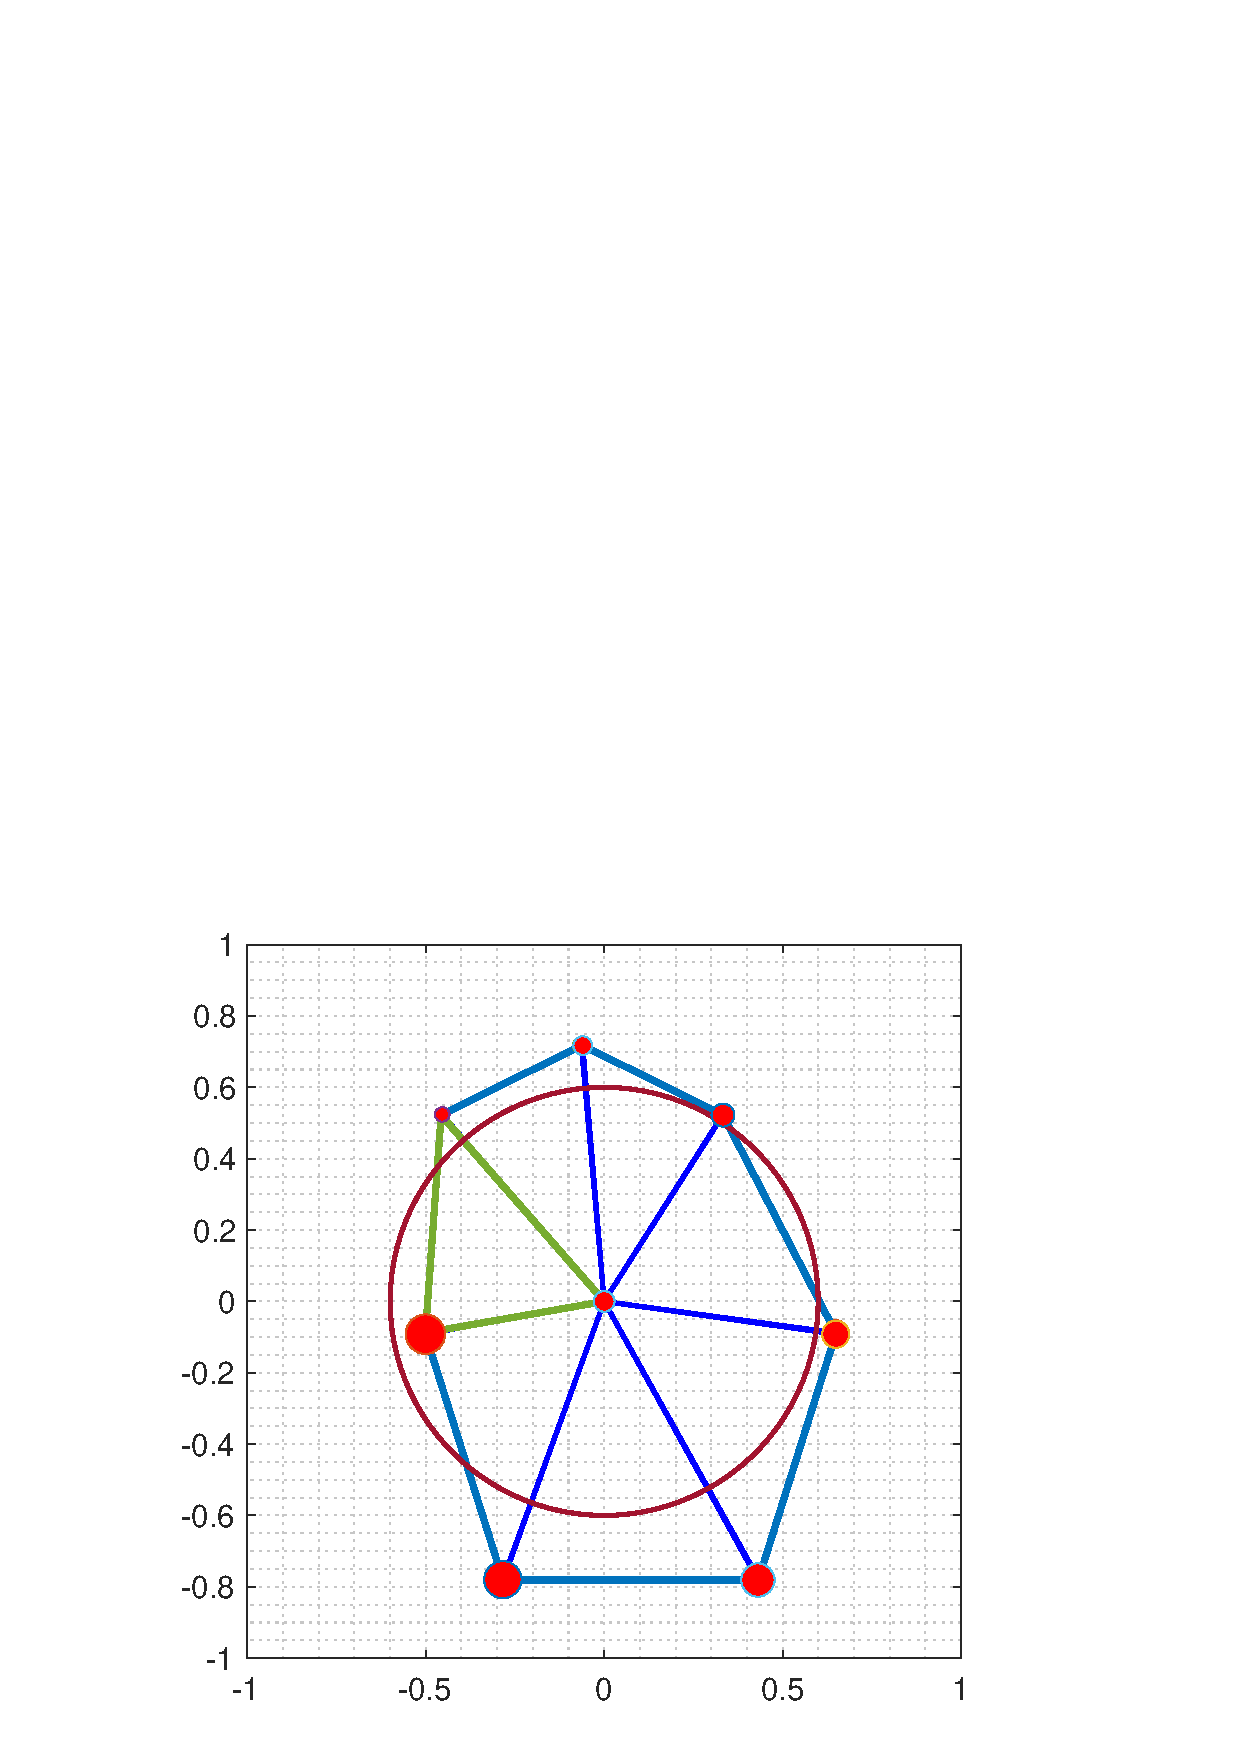
\includegraphics[width=0.8\textwidth]{1.png}
\caption{Representation of the x-axes dynamics system. We can observe the timing pulley, rolling bearing, and timing belt.}
\end{figure}

In the ideal case, using a normal timing pulley, we can say that $\exists K\in \R^+$ s.t. $\Delta w=\Delta \overline{w}=K\Delta u$, representing the lineal relation between the rotation and the belt translation. However, using a non-ideal timing pulley, we have that for very small $\Delta\overline{w}$, there should exists a function $K(\overline{w},\sign(\dot{\overline{w}}),|\dot{\overline{w}}|):[0,2\pi)\times\{0,1\}\times\R\to\R$ s.t. $$\Delta\overline{w}K(\overline{w},\sign(\dot{\overline{w}}),|\dot{\overline{w}}|)=\Delta u.$$

\subsection{Encoder}

Using two encoders we can measure $w(t)$ and $\overline{w}(t)$ during the printing process. We designed a prototype to add encoders to the printer.
\begin{figure}[ht!]
\centering
\includegraphics[width=0.8\textwidth]{20210213_155933.jpg}
\caption{Prototype to test an encoder in the printer's motor.}
\end{figure}

List of possible steps:

\begin{itemize}

\item Once we have the data $w(t)$ and $\overline{w}(t)$, we can simulate a 3D printed model (virtual printer) and measure the error $||\text{REAL 3D MODEL - 3D PRINTED MODEL}||$.

\item As we can control the printer from Python, we may be able to find $K(\overline{w},\sign(\dot{\overline{w}}),|\dot{\overline{w}}|)$ for a fixed $|\dot{\overline{w}}|$. To do this, we map all the function $K(\cdot)$'s domain with Python, and we reconstruct $K(\cdot)$ using the encoders' measurements.

\item Using the encoders we can create a control system to reduce the error.  See Figure \ref{pic2}.
\begin{figure}[ht!]
\centering
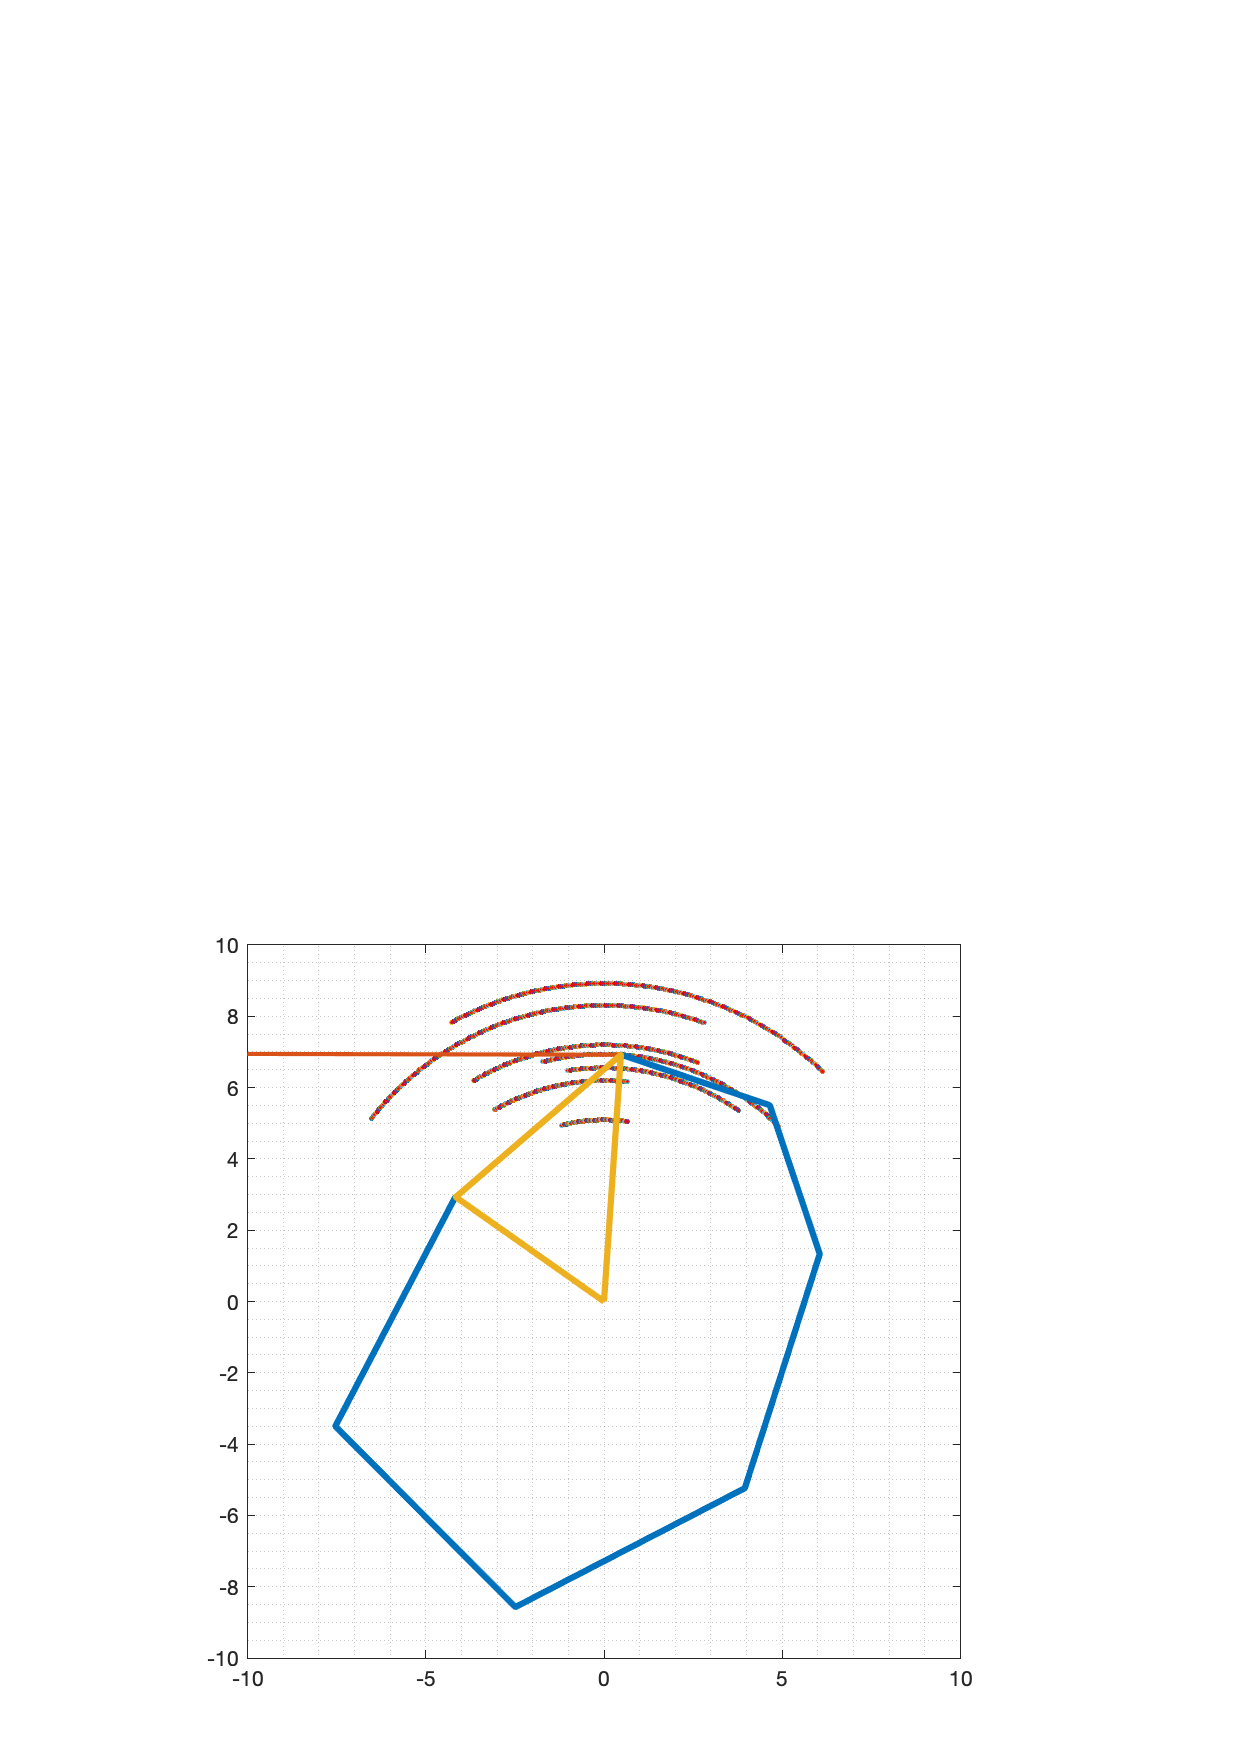
\includegraphics[width=0.8\textwidth]{2.png}
\caption{Possible control system using encoders. The reference can be the g-code.}
\label{pic2}
\end{figure}

\end{itemize}

\subsection{What are we doing right now?}

Still finding the best way to connect encoders to the printer.

\end{document}